\documentclass[12pt]{article}

% packages

%\usepackage{times} % alt: cmbright
\usepackage[top=1in, bottom=1in, left=1in, right=1in]{geometry}
\usepackage{natbib}
\usepackage{amsmath}
\usepackage{amssymb}
\usepackage{latexsym}
\usepackage{sectsty}
\usepackage{amsfonts}
\usepackage{epsfig}
\usepackage{url}
\usepackage{microtype}
\usepackage{fixmath}
\usepackage{hyperref}
\usepackage{amsthm}
\usepackage{subfigure}
\usepackage{float}
\usepackage{hyperref}

\newtheorem{lem}{Lemma}
\newtheorem{defn}{Assumption}
\newtheorem{propty}{Property}
\newtheorem{thm}{Theorem}

% references

\newcommand{\mysec}[1]{Section~\ref{sec:#1}}
\newcommand{\myapp}[1]{Appendix~\ref{app:#1}}
\newcommand{\myeq}[1]{Equation~\ref{eq:#1}}
\newcommand{\myeqp}[1]{Eq.~\ref{eq:#1}}
\newcommand{\mychap}[1]{Chapter~\ref{chap:#1}}
\newcommand{\myfig}[1]{Figure~\ref{fig:#1}}

% math conveniences

\newcommand{\g}{\,\vert\,}
\newcommand{\E}{\textrm{E}}
\newcommand{\vct}[1]{\textbf{#1}}
\newcommand{\realline}{\mathbb{R}}
\newcommand{\indpt}{\protect\mathpalette{\protect\independenT}{\perp}}
\def\independenT#1#2{\mathrel{\rlap{$#1#2$}\mkern2mu{#1#2}}}
\newcommand{\h}[1]{\textrm{H}\left( #1 \right)}
\newcommand{\half}{\frac{1}{2}}
\newcommand{\new}{\textrm{new}}

\newcommand{\mult}{\textrm{Mult}}
\newcommand{\dir}{\textrm{Dir}}
\newcommand{\discrete}{\textrm{Discrete}}
\newcommand{\Bern}{\textrm{Bern}}
\newcommand{\DP}{\textrm{DP}}
\newcommand{\GP}{\textrm{GP}}
\newcommand{\Bet}{\textrm{Beta}}

% paragraph spacing

\setlength{\parindent}{0pt}
\setlength{\parskip}{2ex plus 0.5ex minus 0.2ex}

\allsectionsfont{\sffamily\mdseries}
\paragraphfont{\sffamily\bfseries}

\usepackage{algorithm}
\usepackage{algorithmic}
\renewcommand{\algorithmicrequire}{\textbf{Input:}}
\renewcommand{\algorithmicensure}{\textbf{Output:}}


\begin{document}

\title{\textsf{Semantic-Based Path Planning: A Multi-Objective Optimization Perspective}}
\author{\textsf{Daqing Yi}}
\date{\textsf{Brigham Young University}}

\maketitle

\section{Primitive Objective}

All the path planning leads to an optimization problem, which defines the principles of motion instead of random walking. In the simplest form, a primitive(atomic) optimization problem (indexed as $ i $) can be described as:

\begin{equation}
\label{eq:atomicObj}
\begin{aligned}
\max f_{i}(x) \\
\mbox{s.t. } x \in X_{i}
\end{aligned}
\end{equation}

\section{Multi-Objective Optimization}

In applications, there are usually more than one objective we are interested with. This shapes a multi-objective optimization problem. Because $ \max f(x) $ equals to $ \min -f(x) $, we can combine $ \max $ and $ \min $ in one function. One common way comes to my mind is:

\begin{equation}
\label{eq:severalObjs}
\begin{aligned}
& \max \left[ \gamma_{1} * f_{1}(x) + \gamma_{2} * f_{2}(x) + \cdots + \gamma_{n} * f_{n}(x) \right] \\
& \mbox{s.t. } x \in X_{1} \bigcap X_{2} \cdots \bigcap X_{n} \\
&\gamma_{1} , \gamma_{2} , \cdots , \gamma_{n} \in [0,1]
\end{aligned}
\end{equation}

Apparently that $ \gamma_{1}, \gamma_{2} \cdots \gamma_{n} $ determine how different objectives are weighted.

There is another way to define a multi-objective optimization problem \footnote{\url{http://en.wikipedia.org/wiki/Multi-objective_optimization}}. 

\begin{equation}
\label{eq:multiObjs}
\begin{aligned}
& \max \left( f_{1}(x) , f_{2}(x), \cdots , f_{n}(x)  \right) \\
& \mbox{s.t. } x \in X_{1} \bigcap X_{2} \cdots \bigcap X_{n}
\end{aligned}
\end{equation}

$ \left( f_{1}(x) , f_{2}(x), \cdots , f_{n}(x)  \right) $ is a vector. This shapes the optimal problem that we usually see in multi-agent system. There might exist a \emph{Pareto Optimal Solution} that cannot be improved in any of the objectives without degrading at least one of the other objectives. Also a lot of similar concepts can be imported.

\section{Semantic-Based Path Planning}

\subsection{Semantic-Based Perspective}

A semantic-based Path Planning problem usually gives a more complex scenario, which usually shapes a multi-objective optimization problem rather than a single-objective optimization problem. It is expected that there is a parser that will convert a semantic command to a bunch of primitive objectives, as in Fig.\ref{fig:parser}.

\begin{figure}[hb]
\centering
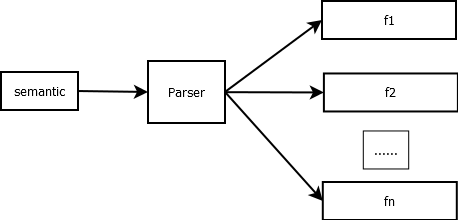
\includegraphics[width=0.7\linewidth]{./parser}
\caption{Semantic Parser}
\label{fig:parser}
\end{figure}

\subsection{Path Planning Perspective}

Path planning gives a sequential optimization problem, in which we need a slight modification on the expression. To normalize different primitive objectives, we define a planning length $ T $ to all the primitive objectives. Thus we have:

\begin{equation}
\label{eq:pathPlanningObj}
\begin{aligned}
& \max f_{i}(x^{1}, x^{2}, \cdots , x^{T}) \\
& \mbox{s.t. } x^{t} \in X_{i}^{t}
\end{aligned}
\end{equation}

In a multi-objective optimization framework, it is written as:

\begin{equation}
\label{eq:pathPlanningMutObj}
\begin{aligned}
& \max \left( f_{1}(x^{1}, x^{2}, \cdots , x^{T}) , f_{2}(x^{1}, x^{2}, \cdots , x^{T}), \cdots , f_{n}(x^{1}, x^{2}, \cdots , x^{T})  \right) \\
& \mbox{s.t. } x^{t} \in X_{1}^{t} \bigcap X_{2}^{t} \cdots \bigcap X_{n}^{t}
\end{aligned}
\end{equation}


\section{A Case Study on our project}

In our project, we are currently interested with five principles in semantic forms, which are ``covertly", ``safely", ``quickly", ``carefully" and ``helpfully". 

\subsection{Atomic}

Firstly, we need to list a set of primitive objectives that we might have interested with.

\begin{itemize}
  \item \textbf{Minimum Visibility} \\
  ``minimize the visibility of the agent through time, $ visibility() $ is the visibility at input position" \\
  objective: $ \min \sum\limits_{1}^{T} visibility(x^{t})  $
  \item \textbf{Minimize Exposure to Dangerous Areas} \\
  ``minimize the reward collected from entering dangerous area, $ danger() $ is the danger collected at input position"
  objective: $ \min \sum\limits_{1}^{T} danger(x^{t}) $
  \item \textbf{Not Seen from Particular Locations} \\
  ``forbidden to get into particular regions"
  constraint: $ \forall t, x^{t} \notin \bigcup_{j} visibility(z^{j}) $
  \item \textbf{Smooth Motion Curve} \\
  ``make the motion as smooth as possible, $ orientation()$ is the orientation calculated from input position"
  objective: $ \min \sum\limits_{1}^{T} \left| orientation(x^{t})-orientation(x^{t-1}) \right| $
  \item \textbf{Obstacle Avoidance} \\
  ``keep away from the obstacle as much as possible, $ obstacle(k) $ is obstacle $ k $"
  objective: $ \min \sum\limits_{1}^{T} \sum\limits_{1}^{k} \left| x^{t} - obstacle(k) \right| $
  \item \textbf{Collision Avoidance} \\
  ``keep away from other moving agent as much as possible, $ agent(l)^{t} $ is agent $ l $ at time $ t $"
  objective: $ \min \sum\limits_{1}^{T} \sum\limits_{1}^{l} \left| x^{t} - agent(l)^{t} \right| $
  \item \textbf{Get to a Specific Position as Closer as Possible} \\
  ``in a limited time, get to a target position as close as possible"
  objective: $ \min \left| x^{T} - targetPosition \right| $
  \item \textbf{Maximize the Information Collection} \\
  ``maximize information collection, $ information() $ is information collected at input position"
  objective: $ \max \sum\limits_{1}^{T}  information(x^{t}) $
  \item \textbf{Wingman Constraint} \\
  ``moving in a proximity of a human, $ y^{t} $ is the human position and $ wingmanArea() $ gives the wingman area by input position"
  constraint: $ \forall t, x^{t} \in wingmanArea(y^{t}) $
\end{itemize}


\subsection{Covertly}

``Covertly" requires a robot keeping avoid of being seen by other agents (teammates and opponents?) Minimizing his own visibility also reduce the chance of being seen.

Under this principle, we are interested with

\begin{itemize}
  \item minimum visibility 
\end{itemize}

\subsection{Safely}

``Safely" expects a robot keeping away from dangerous areas and not being seen from particular locations.

Under this principle, we are interested with

\begin{itemize}
  \item minimize exposure to dangerous areas,
  \item not seen from particular locations.
\end{itemize}

\subsection{Quickly}

``Quickly" means a robot should try to get to a target position as soon as possible. 

Under this principle, we are interested with

\begin{itemize}
  \item get to a specific position as closer as possible.
\end{itemize}

\subsection{Carefully}

``Carefully" shows that a robot should take a steady and smooth motion and be avoid of colliding with any object. This might be used when a robot is carrying something important.

Under this principle, we are interested with

\begin{itemize}
  \item smooth motion curve,
  \item obstacle avoidance,
  \item collision avoidance.
\end{itemize}

\subsection{Helpfully}

``Helpfully" assigns a role of assisting human to a robot. He should cooperate the work of a human and be responsive to any requirement.

Under this principle, we are interested with

\begin{itemize}
  \item maximize the information collection,
  \item motion under wingman constraint.
\end{itemize}

\subsection{Semantic Ontology}

Some examples are given in XML format. The relationship can also be described by chart, as in Fig.\ref{fig:class1} and Fig.\ref{fig:class2}.

\lstset{language=XML}
\begin{lstlisting}
<?xml version="1.0"?>
<rdf:Description rdf:about="#Careful"> 
   <hasPrimitive rdf:resource="#smooth motion curve" /> 
   <hasPrimitive rdf:resource="#obstacle avoidance" /> 
   <hasPrimitive rdf:resource="#collision avoidance" />
</rdf:Description>
\end{lstlisting}

\begin{lstlisting}
<rdf:Description rdf:about="#smooth motion curve">
   <objective from="1" to="T" operator="sum">
    | orientation(x^{t})-orientation(x^{t-1}) |
   </objective>
   </constraint>
</rdf:Description>

<rdf:Description rdf:about="#get to a specific position as closer as possible">
   <objective from="T" to="T" operator="sum">
       | x^{t} - targetPosition |
      </objective>
   </constraint>
</rdf:Description>

<rdf:Description rdf:about="#wingman constraint">
   </objective>
   <constraint from="1" to="T" type="in">
   wingmanArea(y^{t})
   </constraint>
</rdf:Description>
\end{lstlisting}


\begin{figure}[htbp]
\centering
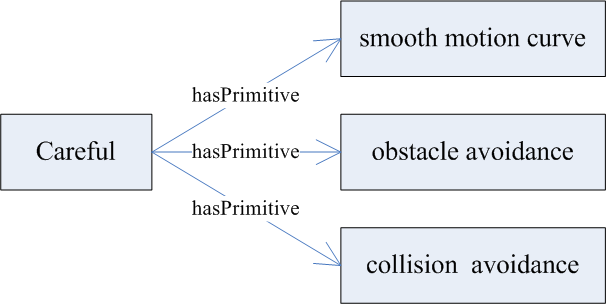
\includegraphics[width=0.4\textwidth]{./class1}
\caption{the class of "Careful"}
\label{fig:class1}
\end{figure}

\begin{figure}[htbp]
\centering
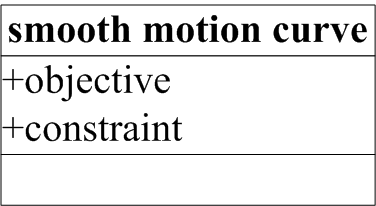
\includegraphics[width=0.3\textwidth]{./class2}
\caption{the class of "smooth motion curve"}
\label{fig:class2}
\end{figure}


\bibliographystyle{apalike}
\bibliography{bib}

\end{document}
